\chapter{Exercícios}

\begin{exercicio}
  {2º/2017}{\textit{Threads}}
  {Por quê a implementação de \textit{threads} em nível de usuário possui um custo extremamente baixo de troca de contexto?}

  Resposta aqui
\end{exercicio}

\begin{exercicio}
  {2º/2017}{Condições de Corrida}
  {Considere o código multi-processo abaixo. Existe condição de corrida nesse código? Se sim, corrija o código de maneira a eliminá-la.}


\end{exercicio}

\begin{exercicio}
  {2º/2017}{\textit{Deadlocks}}
  {Por quê \textit{deadlocks} são ditos \textit{stable properties}?}


\end{exercicio}

\begin{exercicio}
  {2º/2017}{Arquivos}
  {Qual a função da operação \texttt{OPEN} e \texttt{CLOSE}?}

  \texttt{OPEN:} fazer a associação entre o processo e o arquivo, através da tabela de descritores, retornando um descritor que será usado nas próximas operações.

  \texttt{CLOSE}: desfazer a associação entre processo e arquivo, tornando o descritor indisponível.
\end{exercicio}

\begin{exercicio}
  {2º/2017}{Memória Virtual}
  {
    Considere um sistema de memória virtual paginada. Dê os nomes dos elementos marcados com (a), (b), (c) e (d) na figura abaixo e explique como cada um é utilizado em uma operação de acesso à memória.
    % \begin{figure}
    %   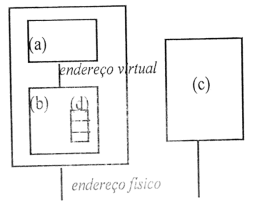
\includegraphics[0.4\textwidth]{ex-mem-structure}
    % \end{figure}
  }

  \begin{enumerate}[label=(\alph*)]
    \item \textbf{CPU:} envia o endereço virtual à MMU;

    \item \textbf{MMU:} quebra o endereço virtual em duas partes, sendo elas a página e o deslocamento. A MMU usa $p$ como índice na TLB para obter o \textit{frame} $f$. A MMU troca a página $p$ pelo frame $f$, que é jogado no barramento junto com o deslocamento.

    \item \textbf{Memória RAM:} entidade que guarda o dado desejado e será acessada;

    \item \textbf{Tabela de Páginas:} guarda % TODO: completar
  \end{enumerate}
\end{exercicio}


\begin{exercicio}
  {2º/2017}{Paginação}
  {Considere um sistema com 4 \textit{frames} e 8 páginas. Admita a seguinte \textit{string} de referência: 0172327103. Quantos \textit{page faults} ocorrerão se o algorítmo de substituição for FIFO? E se for LRU?}

  Fazer o exercício de forma a mostrar cada iteração e o histórico das tabelas.

  FIFO: 6 page faults

  LRU: 7 page faults
\end{exercicio}

\begin{exercicio}
  {2º/2017}{Arquiteturas de SO/Processos}
  {Cite os passos para a criação de processos nas arquiteturas monolíticas, \textit{microkernel} e \textit{exokernel}.}

  Para as \textsc{arquiteturas monolíticas}:
  \begin{enumerate}
    \item O processo pai solicita a criação de um processo filho, através de uma \textit{chamada de sistema} \texttt{create process};

    \item O SO aloca uma entrada livre na \textit{tabela de processos} para o processo filho;

    \item O SO atribui um \textit{PID} ao processo filho;

    \item O SO ajusta a \textit{área de memória} para a execução do processo filho;
    \begin{itemize}
      \item % TODO: o que faz quando é criação tradicional?
      \item % TODO: o que faz quando é clonagem?
    \end{itemize}

    \item O SO preenche os \textit{valores de registradores} para execução do processo filho na tabela de processos;

    \item O SO insere o processo filho na fila \textit{ready} do escalonador;

    \item O SO retorna ao processo pai.
  \end{enumerate}

  Para o \textsc{microkernel}:
  \begin{enumerate}
    \item O processo pai envia uma mensagem para o microkernel, colocando o \texttt{create process} como conteúdo;

    \item O microkernel recebe a mensagem e determina que o processo filho deve ser criado;

    \item O microkernel aloca uma entrada livre na \textit{tabela de processos} para o processo filho;

    \item O microkernel atribui um \textit{PID} ao processo filho;

    \item O microkernel ajusta a \textit{área de memória} para a execução do processo filho;

    \item O microkernel preenche os \textit{valores de registradores} para execução do processo filho na tabela de processos;

    \item O microkernel insere o processo filho na fila \textit{ready} do escalonador;

    \item O microkernel envia uma mensagem para o processo pai contendo o valor de retorno.
  \end{enumerate}

  Para o \textsc{exokernel}:
  \begin{enumerate}
    \item O processo pai solicita a criação de um processo filho para a LibOS, através de uma \textit{chamada de função} \texttt{create process};

    \item A LibOS aloca uma entrada livre na \textit{tabela de processos} para o processo filho;

    \item A LibOS atribui um \textit{PID} ao processo filho;

    \item A LibOS pede uma região de software (área de memória) ao exokernel, via \textit{chamada de sistema}. Esta área é destinada ao processo filho;

    \item A LibOS solicita um \textit{processor environment} (PE), via chamada de sistema, e copiar o valor dos registradores para lá;

    \item A LibOS preenche o de prólogo e epílogo do PE (troca de contexto), descarregando o código;

    \item O exokernel coloca o PE na sua fila \textit{ready};

    \item A LibOS coloca o processo na sua fila \textit{ready};

    \item A LibOS retorna ao processo pai.
  \end{enumerate}

\end{exercicio}
